\chapter{\label{cha:results}Results}

This chapter presents the empirical findings of the thesis. It is split
into two parts: a study of discretization invariance for FNO and CNO,
and an investigation of geo-FNO on non-uniform meshes, including its
application to a nuclear dataset.

\section{Part I: Discretization Invariance Study}

\begin{figure}
    \centering
    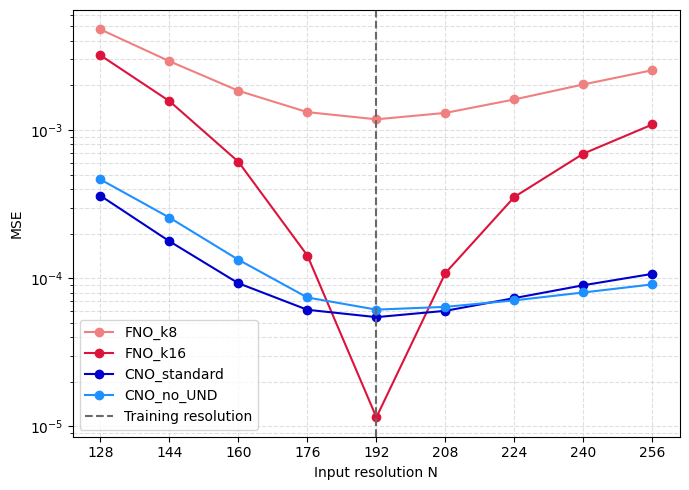
\includegraphics[width=0.8\textwidth]{figures/loss_vs_resolution_navier_stokes.png}
    \caption{\label{fig:loss_vs_resolution_navier_stokes} A plot of the MSE loss as a function of resolution for the four models trained on the Navier-Stokes dataset. The training resolution is indicated by the vertical dashed line.}
\end{figure}

\begin{figure}
    \centering
    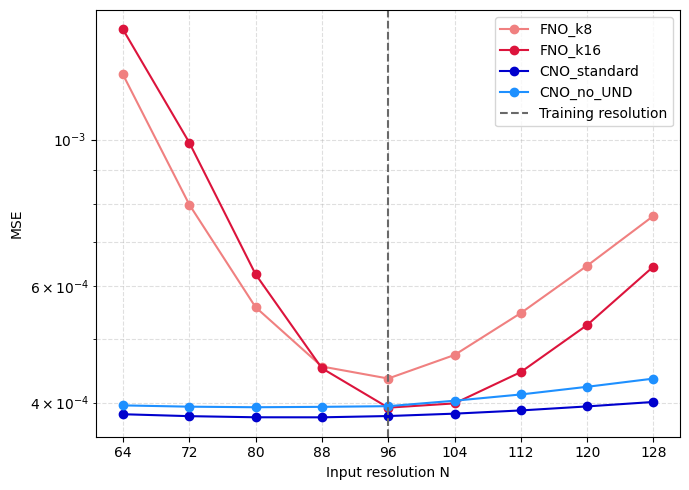
\includegraphics[width=0.8\textwidth]{figures/loss_vs_resolution_darcy_flow.png}
    \caption{\label{fig:loss_vs_resolution_darcy_flow} A plot of the MSE loss as a function of resolution for the four models trained on the Darcy flow dataset. The training resolution is indicated by the vertical dashed line.}
\end{figure}

\begin{table}
    \centering
    \caption{\label{tab:di-values} Discretization robustness score $D$ for the uniform-grid experiments. Lower values indicate that the loss remains more consistent across evaluation resolutions relative to the loss at the training resolution.}
    \begin{tabular}{lcc}
        \hline
        Model & Navier-Stokes & Darcy flow \\
        \hline
        FNO\_k8 & 0.5076 & 0.3583 \\
        FNO\_k16 & 3.4817 & 0.4179 \\
        CNO\_standard & 0.5854 & 0.0140 \\
        CNO\_no\_UND & 0.5847 & 0.0260 \\
        \hline
    \end{tabular}
\end{table}

\subsection{FNO versus CNO}

\subsubsection{Results}

Present the quantitative comparison between FNO and CNO and discuss how
performance changes under resolution transfer.

\subsection{Interpretation of discretization effects}

This section should connect the observations back to the theoretical
differences between the models.

\subsubsection{FNO}

Discuss spectral truncation and the fact that Fourier mode index does
not preserve the same physical meaning when the discretization changes.

\subsubsection{CNO}

Discuss the role of locality, the bandlimited assumption, and the
implicit multiscale structure in producing steadier behavior across
resolutions.

\subsubsection{Connection to theory}

Tie the empirical behavior back to the contrast between bandlimiting
and Fourier truncation.

\section{Part II: Non-uniform Meshes and geo-FNO}

\subsection{Results}

Present the geo-FNO results on the irregular-domain datasets and
discuss the overall performance.

\subsection{Analysis of seam artifacts}

This section can document the seam artifact, explain how it manifests in
different datasets, and analyze why some datasets are more robust to it
than others.

\subsubsection{Observed artifact}

Describe the seam, the associated corruption of low-$k_x$ modes, and
the evidence that it appears across datasets.

\subsubsection{Tracing the source}

Explain how the issue was traced to the \texttt{conv0} layer and what
was ruled out during debugging, including the approximate
\texttt{fft2d}/\texttt{ifft2d} functions and the handling of complex
weights.

\subsubsection{Patch and effect}

Explain the bug in the original implementation, how it was fixed, and
show the before-and-after effect of the patch.

\subsection{Nuclear application}

Describe the nuclear dataset, explain the prediction task, and discuss
how geo-FNO performs on unseen $z$ levels and temperatures.

\subsubsection{Dataset characteristics}

Explain why the dataset is relatively simple and consider supporting
that claim with a PCA visualization.

\subsubsection{Generalization results}

Discuss the extent to which the experiment demonstrates that geo-FNO
extends to nuclear applications.

\section{Writing note}

An open presentation choice is whether to show the original seam-affected
plots in the main text before introducing the patch, or to present only
the corrected results in the main text and move most debugging evidence
to an appendix.

